\documentclass[20pt]{article}
\usepackage[T2A]{fontenc}
\usepackage{mathtools}
\usepackage[utf8]{inputenc}
\usepackage[english, russian]{babel}
\usepackage{fancyhdr}
\usepackage{graphicx}
\usepackage{gensymb}
\usepackage{floatrow}
\usepackage{amssymb}
\usepackage{multirow}

\pagestyle{fancy}
\author{}
\title{Определение теплопроводности газов при атмосферном давлении}
\lhead{Работа 2.2.3}
\rhead{Терехов Максим 876}
\date{}

\begin{document}
\selectlanguage{russian}
\parindent=1cm
\large
\maketitle
\section{Цель работы:}
определение коэффициента теплопроводности воздуха или углекислого газа при атмосферном давлении и разных температурах по теплоотдаче нагреваемой током нити в цилиндрическом сосуде.
\section{В работе используются:}
прибор для определения теплопроводности газов; форвакуумный насос; газгольдер с углекислым газом; манометр; магазин сопротивлений; эталонное сопротивление 10 Ом; цифровой вольтметр В7-38; источник питания.
\section{Экспериментальная установка:}
\begin{figure}[H]
	\centering
	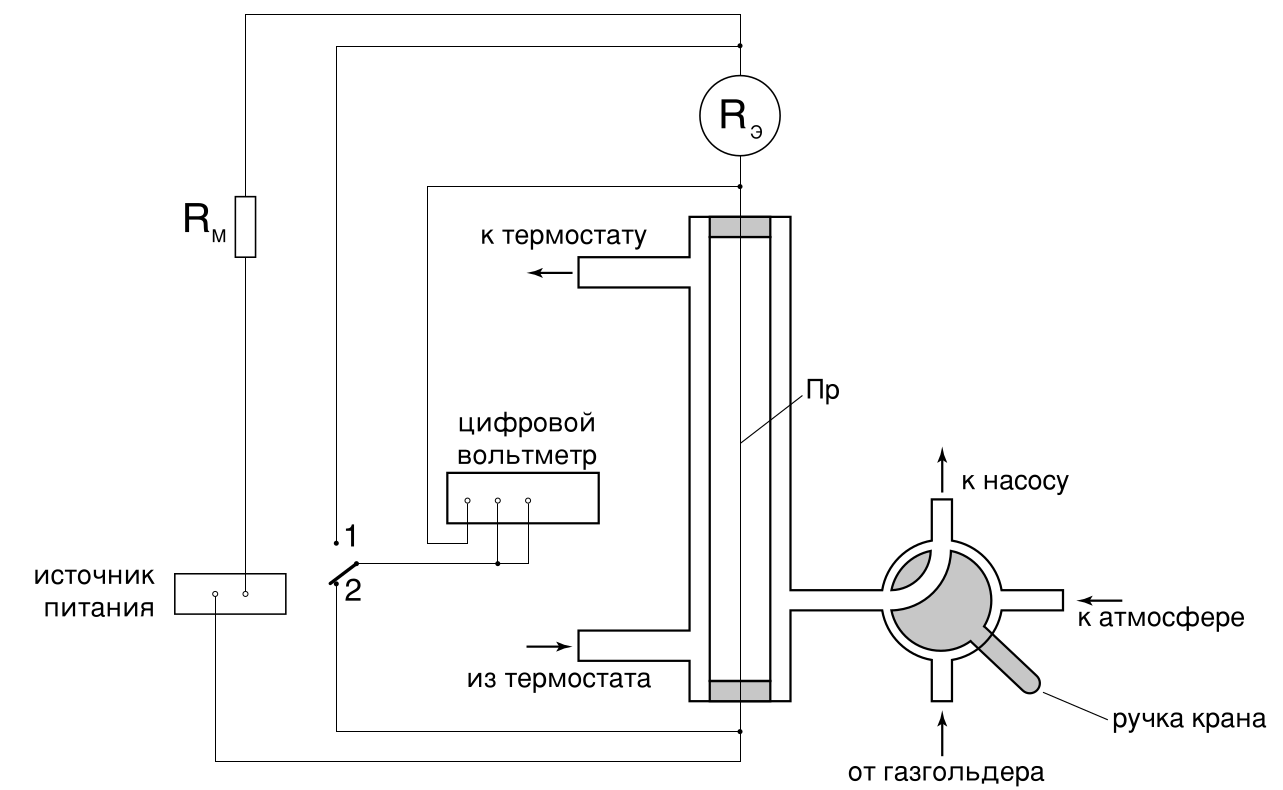
\includegraphics[scale=0.25]{asd.png}
\end{figure}
\section{Теоретическая часть:}
Если температура заключенного в сосуд газа зависит от координат, в газе возникают процессы, приводящие к выравниванию температуры. В обычных условиях среди этих процессов наибольшую роль играет конвекция. Конвекция появляется из-за того, что легкий
теплый газ поднимается вверх, а на его место опускаются более холодные массы газа. Конвекция не возникает, если температура газа
повышается с высотой, если объем газа невелик или если он разбит на небольшие каналы или ячейки. В последних двух случаях возникновению конвекционных потоков мешает вязкость.

При отсутствии конвекции процесс переноса тепла замедляется, но не прекращается. Он происходит благодаря теплопроводности газа, связанной с тепловым движением молекул. Выравнивание температуры получается при этом из-за непрерывного перемешивания
«горячих» и «холодных» молекул, происходящего в процессе их теплового движения и не сопровождающегося макроскопическими перемещениями газа. Нас будет интересовать именно этот случай.

Для цилиндрически симметричной установки, в которой поток
тепла направлен к стенкам цилиндра от нити, расположенной по его
оси, справедлива формула:
\[
	\varkappa = \frac{Q}{T_1-T_2} \frac{1}{2\pi L} =  \frac{dQ}{dR} \frac{dR}{dT} \frac{1}{2\pi L},
\]
где $\varkappa$ --- коэффициент теплопроводности, $Q$ --- выделяемая мощность, $r_1$ и $r_2$ --- радиусы нити и внешнего цилиндра соответственно, $L$ --- длина нити.
\section{Обработка результатов измерений:}

\begin{tabular}{|c|c|c|c|}

\hline $L, \text{мм}$ & $2r_1, \text{мм}$ & $2r_2, \text{мм}$ & $R_{\text{э}}, \text{Ом}$ 
\\\hline $367$ & $0.05$ & $10$ & $10$ \\\hline
\end{tabular}

Для каждого измерения найдем ток, мощность, выделяемую в нити и сопротивление нити по формулам:
\[
	I = \frac{U_{\text{э}}}{R_0}
\]
\[
	Q = I U_{\text{н}} = U_{\text{н}} \frac{U_{\text{э}}}{R_{\text{э}}} 
\]
\[
	R_\text{н} = \frac{U_\text{н}}{I} = \frac{U_\text{э}}{U_\text{э}}
\]
\begin{tabular}{|c|c|c|c|c|c|}
\hline $T, K$ & $U_\text{э}, \text{мВ}$ & $U_{\text{н}}, \text{мВ}$ & $I, \text{мА}$ & $Q, \text{мВт}$ & $R_{\text{н}}, \text{Ом}$ \\\hline
\multirow{8}{*}{297.5}
 & $119.5$ & $1803.3$ & $11.95$ & $12.96$ & $150.9$ \\\cline{2-6}
 & $129.1$ & $1949.7$ & $12.91$ & $25.17$ & $151.0$ \\\cline{2-6}
 & $170.1$ & $2571.3$ & $17.01$ & $43.72$ & $151.2$ \\\cline{2-6}
 & $200.0$ & $3028.2$ & $20.00$ & $60.56$ & $151.4$ \\\cline{2-6}
 & $224.5$ & $3403.4$ & $22.45$ & $76.41$ & $151.6$ \\\cline{2-6}
 & $246.4$ & $3740.3$ & $24.64$ & $92.16$ & $151.8$ \\\cline{2-6}
 & $264.9$ & $4025.9$ & $26.49$ & $106.67$ & $151.9$ \\\cline{2-6}
 & $283.5$ & $4312.3$ & $28.35$ & $122.25$ & $152.1$ \\\hline
\end{tabular} \\\\\\
\begin{tabular}{|c|c|c|c|c|c|}
\hline $T, K$ & $U_\text{э}, \text{мВ}$ & $U_{\text{н}}, \text{мВ}$ & $I, \text{мА}$ & $Q, \text{мВт}$ & $R_{\text{н}}, \text{Ом}$ \\\hline
\multirow{8}{*}{308}
 & $100.1$ & $1525.4$ & $10.01$ & $15.27$ & $152.3$ \\\cline{2-6}
 & $139.1$ & $2121.4$ & $13.91$ & $29.51$ & $152.4$ \\\cline{2-6}
 & $170.8$ & $2608.3$ & $17.08$ & $44.56$ & $152.6$ \\\cline{2-6}
 & $204.3$ & $3095.7$ & $20.43$ & $64.31$ & $152.8$ \\\cline{2-6}
 & $221.3$ & $3385.8$ & $22.13$ & $74.92$ & $152.9$ \\\cline{2-6}
 & $241.1$ & $3692.7$ & $24.11$ & $89.04$ & $153.1$ \\\cline{2-6}
 & $260.5$ & $3994.1$ & $26.05$ & $104.04$ & $153.3$ \\\cline{2-6}
 & $275.7$ & $4230.3$ & $27.57$ & $116.62$ & $153.4$ \\\hline
\end{tabular} \\\\\\
\begin{tabular}{|c|c|c|c|c|c|}
\hline $T, K$ & $U_\text{э}, \text{мВ}$ & $U_{\text{н}}, \text{мВ}$ & $I, \text{мА}$ & $Q, \text{мВт}$ & $R_{\text{н}}, \text{Ом}$ \\\hline
\multirow{8}{*}{318}
 & $98.0$ & $1506.5$ & $9.80$ & $14.77$ & $153.7$ \\\cline{2-6}
 & $140.9$ & $2169.2$ & $14.9$ & $30.58$ & $153.9$ \\\cline{2-6}
 & $170.9$ & $2632.4$ & $17.09$ & $44.98$ & $154.0$ \\\cline{2-6}
 & $190.7$ & $2940.0$ & $19.07$ & $56.07$ & $154.1$ \\\cline{2-6}
 & $220.5$ & $3403.0$ & $22.05$ & $75.01$ & $154.3$ \\\cline{2-6}
 & $240.1$ & $3710.1$ & $24.01$ & $89.09$ & $154.5$ \\\cline{2-6}
 & $260.2$ & $4024.6$ & $26.02$ & $104.72$ & $154.7$ \\\cline{2-6}
 & $275.2$ & $4260.8$ & $27.52$ & $117.28$ & $154.8$ \\\hline
\end{tabular} \\\\\\
\begin{tabular}{|c|c|c|c|c|c|}
\hline $T, K$ & $U_\text{э}, \text{мВ}$ & $U_{\text{н}}, \text{мВ}$ & $I, \text{мА}$ & $Q, \text{мВт}$ & $R_{\text{н}}, \text{Ом}$ \\\hline
\multirow{8}{*}{328}
 & $98.1$ & $1521.1$ & $9.81$ & $14.92$ & $155.1$ \\\cline{2-6}
 & $139.2$ & $2160.4$ & $13.92$ & $30.07$ & $155.2$ \\\cline{2-6}
 & $170.0$ & $2642.4$ & $17.00$ & $44.93$ & $155.4$ \\\cline{2-6}
 & $196.1$ & $3050.6$ & $19.61$ & $59.83$ & $155.5$ \\\cline{2-6}
 & $219.0$ & $3410.6$ & $21.90$ & $74.69$ & $155.7$ \\\cline{2-6}
 & $240.6$ & $3749.9$ & $24.06$ & $90.22$ & $155.8$ \\\cline{2-6}
 & $259.1$ & $4042.0$ & $25.91$ & $104.72$ & $156.0$ \\\cline{2-6}
 & $274.9$ & $4292.7$ & $27.49$ & $118.01$ & $156.1$ \\\hline
\end{tabular} \\\\\\
\begin{tabular}{|c|c|c|c|c|c|}
\hline $T, K$ & $U_\text{э}, \text{мВ}$ & $U_{\text{н}}, \text{мВ}$ & $I, \text{мА}$ & $Q, \text{мВт}$ & $R_{\text{н}}, \text{Ом}$ \\\hline
\multirow{8}{*}{338}
 & $98.0$ & $1533.9$ & $9.80$ & $15.04$ & $156.4$ \\\cline{2-6}
 & $139.2$ & $2160.4$ & $13.92$ & $30.07$ & $156.5$ \\\cline{2-6}
 & $169.2$ & $2652.3$ & $16.92$ & $44.87$ & $156.7$ \\\cline{2-6}
 & $195.0$ & $3059.6$ & $19.50$ & $59.66$ & $156.9$ \\\cline{2-6}
 & $218.2$ & $3427.1$ & $21.82$ & $74.78$ & $157.0$ \\\cline{2-6}
 & $239.6$ & $3767.1$ & $23.96$ & $90.27$ & $157.2$ \\\cline{2-6}
 & $258.8$ & $4073.4$ & $25.88$ & $105.39$ & $157.3$ \\\cline{2-6}
 & $278.7$ & $4309.7$ & $27.87$ & $117.94$ & $157.5$ \\\hline
\end{tabular}\\
Построим график зависимости сопротивления нити от температуры и из наклона графика найдём $dR/dT$:
\begin{figure}[H]
	\centering
	\caption{Зависимость сопротивления нити от температуры}
	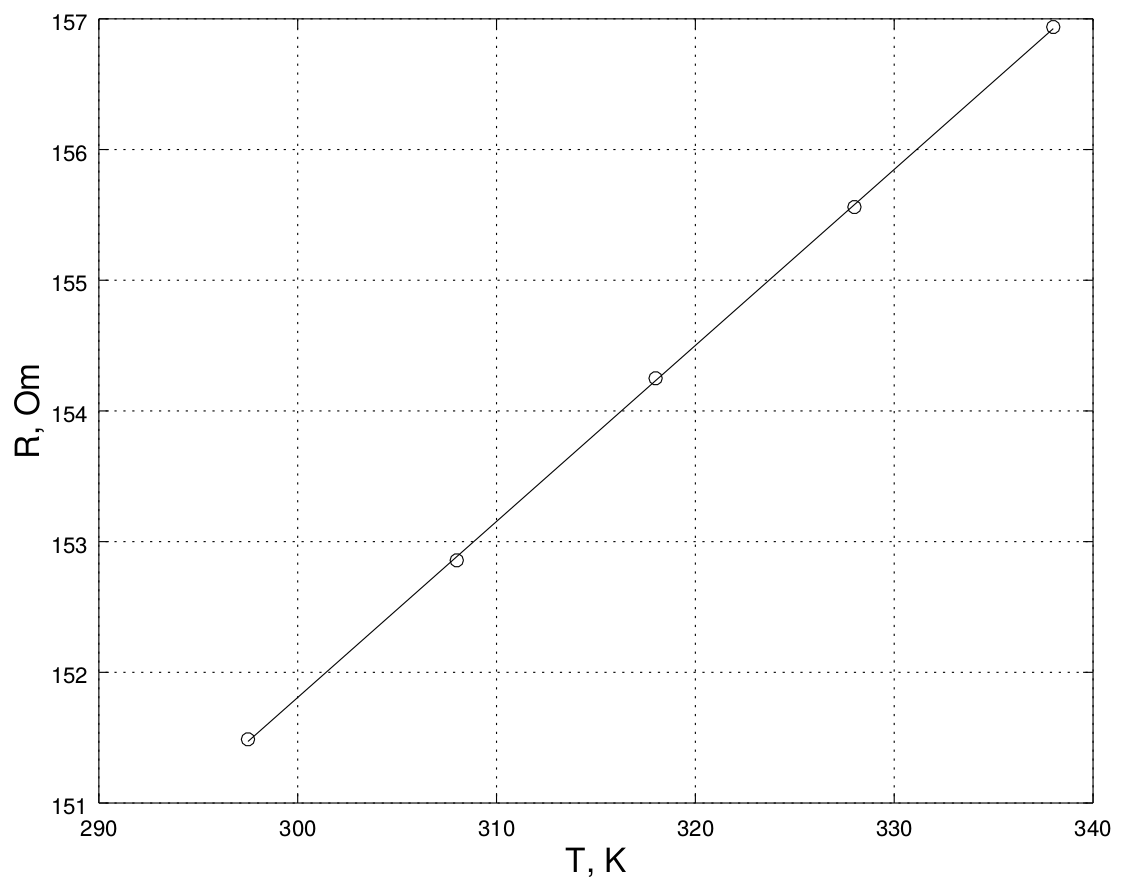
\includegraphics[scale=0.25]{rt.png}
\end{figure}
Как видно, точки хорошо ложатся на прямую.
\[
	\frac{dR}{dT} = 0.13468 
\]
Посчитаем температурный коэффициент сопротивления материала нити:
\[
	\alpha = \frac{1}{R_{273}} \frac{dR}{dT} = 0.9 \cdot 10^{-3} K^{-1}
\]
Построим для каждого $T$ графики зависимости $Q$ от $R$ и из наклонов графиков найдём $dQ/dT$:
\begin{figure}[H]
	\centering
	\caption{Зависимость $Q$ от $R$ при $T_1$}
	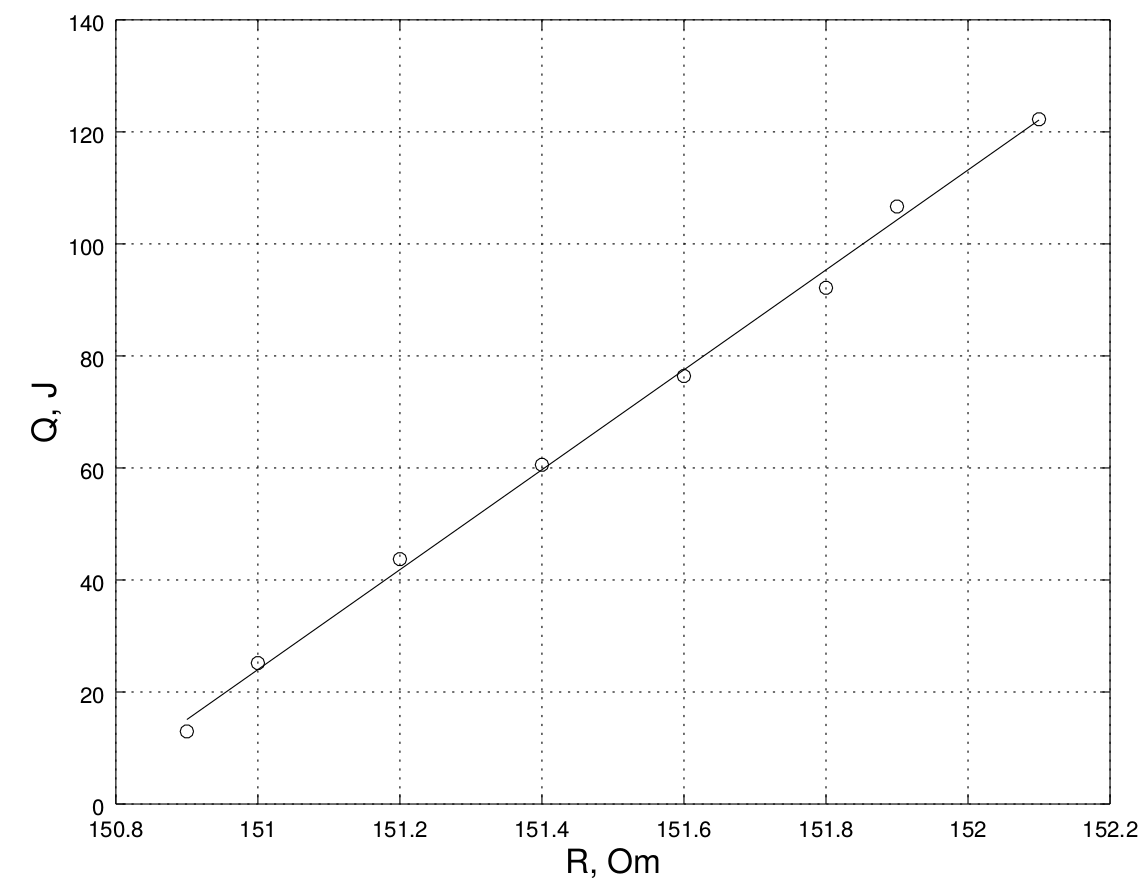
\includegraphics[scale=0.25]{t1.png}
\end{figure}
\begin{figure}[H]
	\centering
	\caption{Зависимость $Q$ от $R$ при $T_2$}
	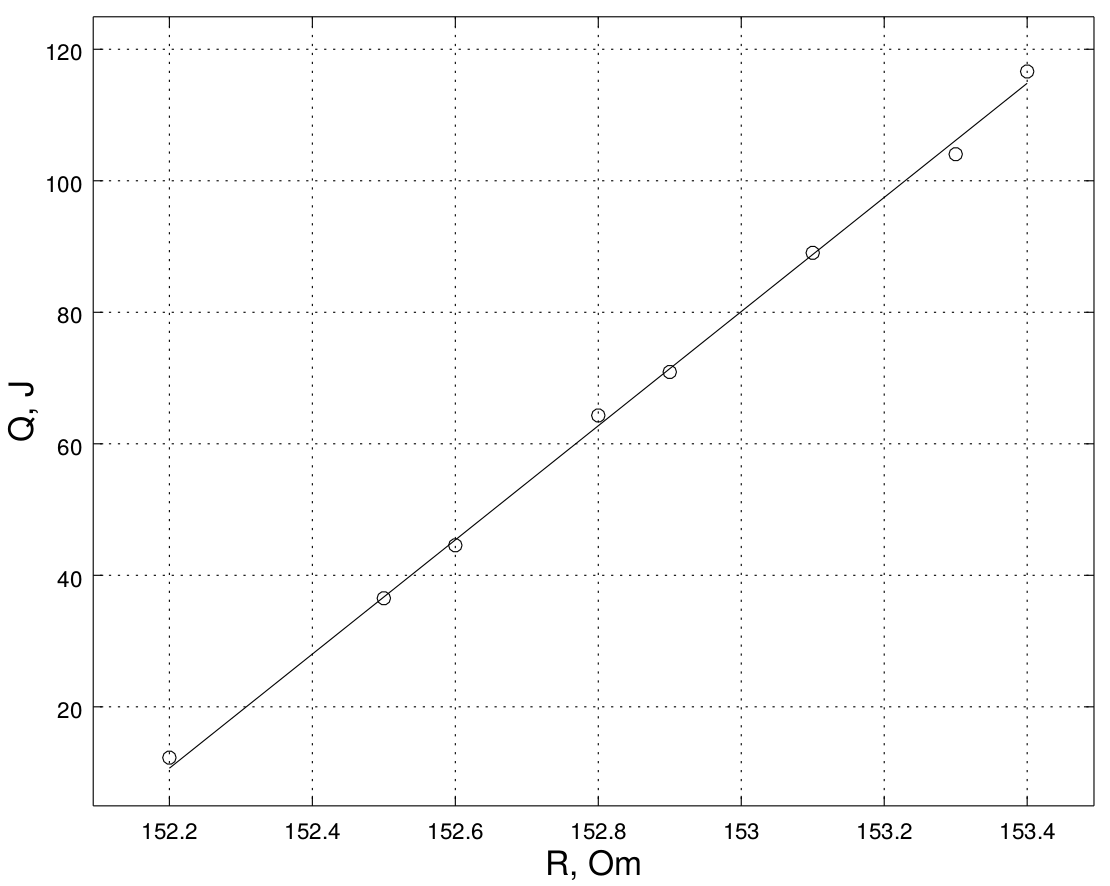
\includegraphics[scale=0.25]{t2.png}
\end{figure}
\begin{figure}[H]
	\centering
	\caption{Зависимость $Q$ от $R$ при $T_3$}
	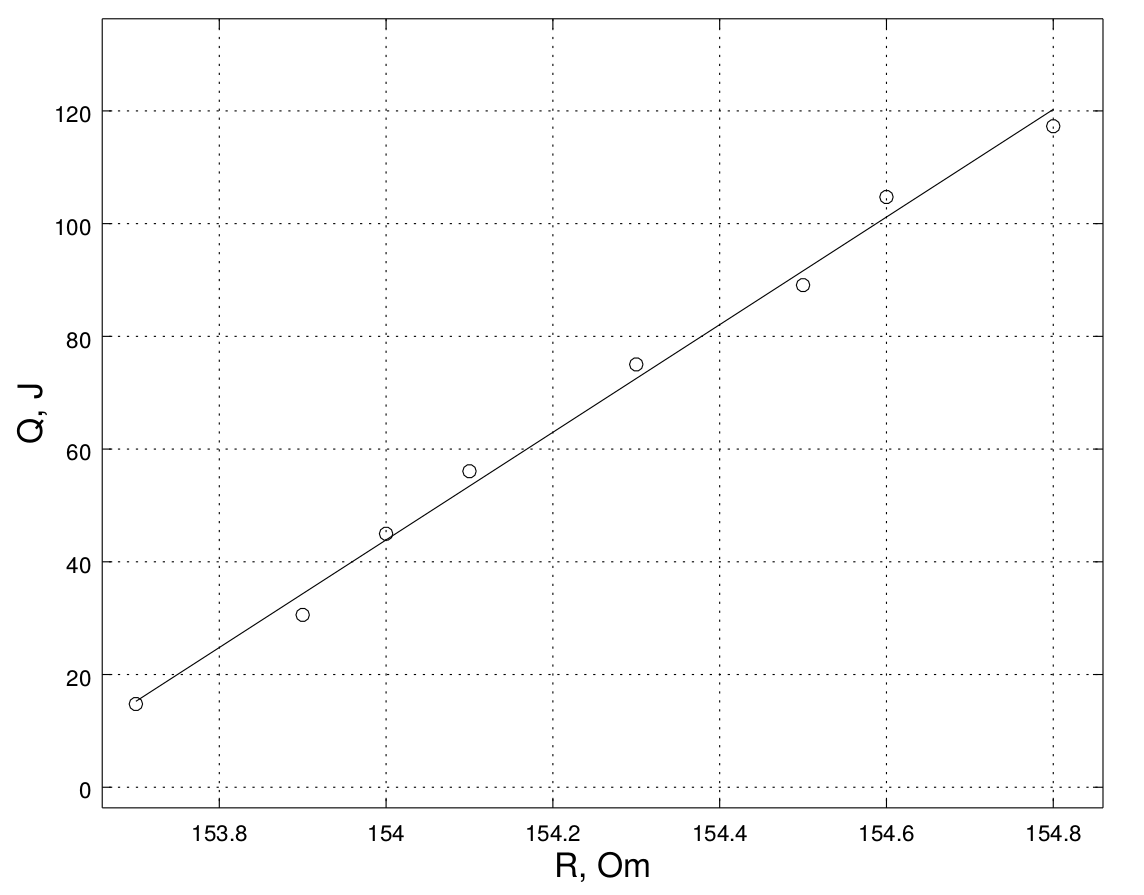
\includegraphics[scale=0.25]{t3.png}
\end{figure}\begin{figure}[H]
	\centering
	\caption{Зависимость $Q$ от $R$ при $T_4$}
	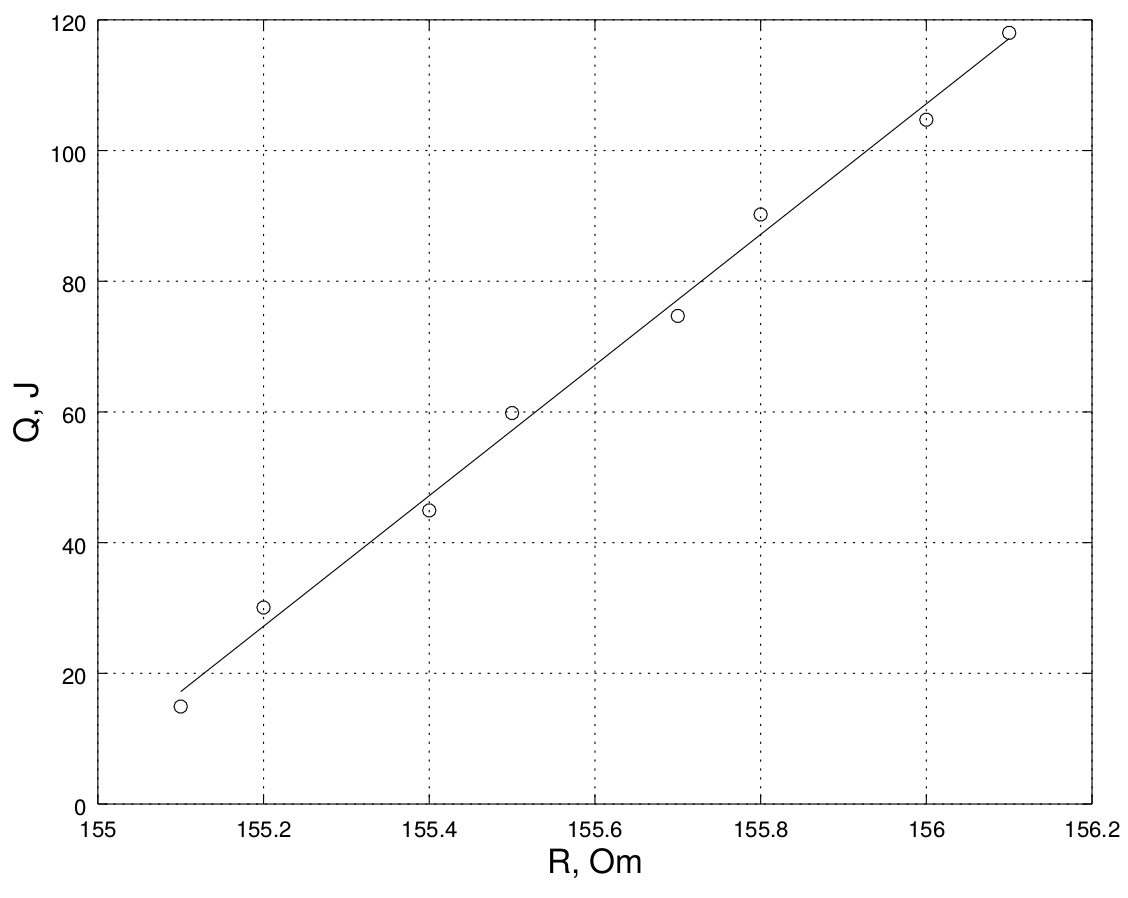
\includegraphics[scale=0.25]{t4.png}
\end{figure}\begin{figure}[H]
	\centering
	\caption{Зависимость $Q$ от $R$ при $T_5$}
	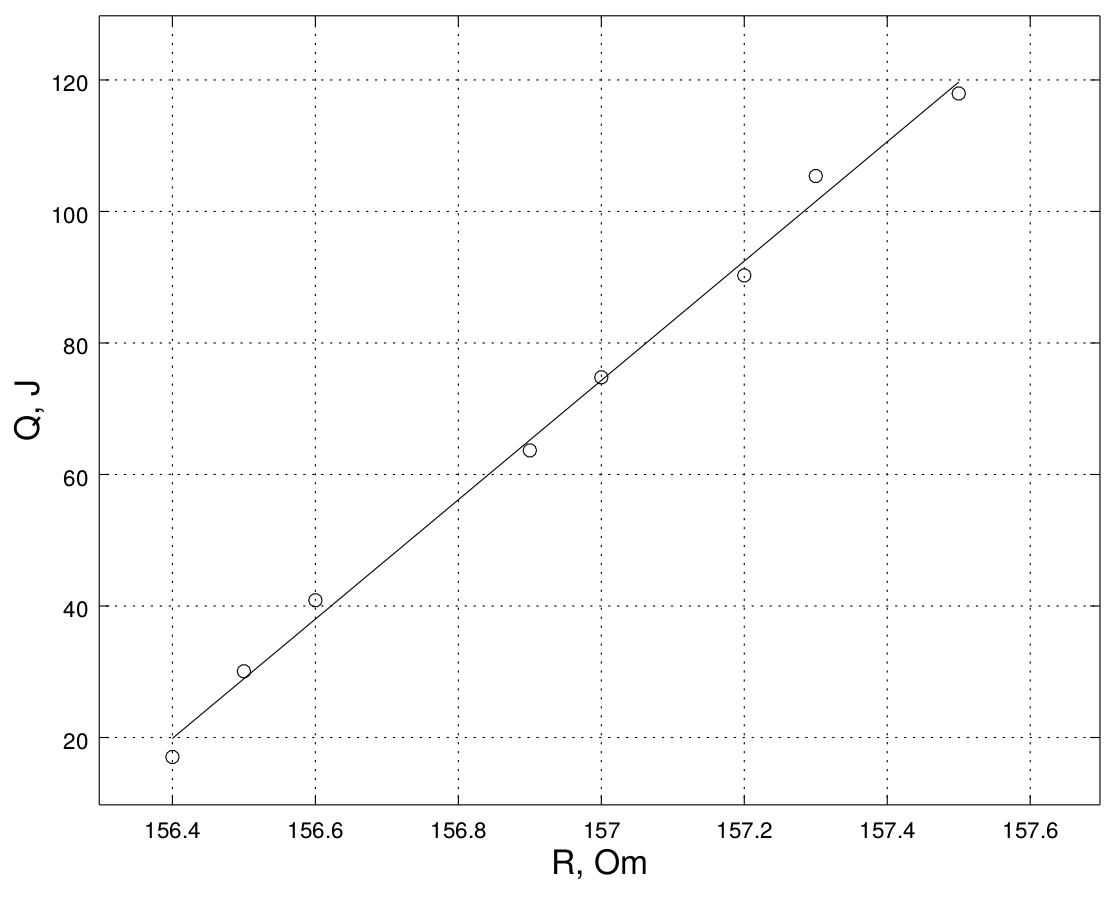
\includegraphics[scale=0.25]{t5.png}
\end{figure}
\begin{tabular}{|c|c|c|c|c|c|}
\hline
$T, K$ & $297.5$ & $308$ & $318$ & $328$ & $338$    \\\hline	
$\frac{dQ_1}{dT},\ \frac{\text{Дж}}{K}$ & $0.0120$ & $0.0125$ & $0.0129$ & $0.0134$ & $0.0140$  \\\hline
$\varkappa, \frac{\text{Вт}}{\text{м}}$ & $25.98 \pm 0.9$ & $26.62 \pm 1.0$ & $27.74 \pm 1.1$ & $28.55 \pm 1.1$ & $29.84 \pm 1.2$ \\\hline 
\\
\end{tabular}
Построим график $\ln\varkappa$ от $\ln T$:
\begin{figure}[H]
	\centering
	\caption{Зависимость $\ln\varkappa$ от $\ln T$}
	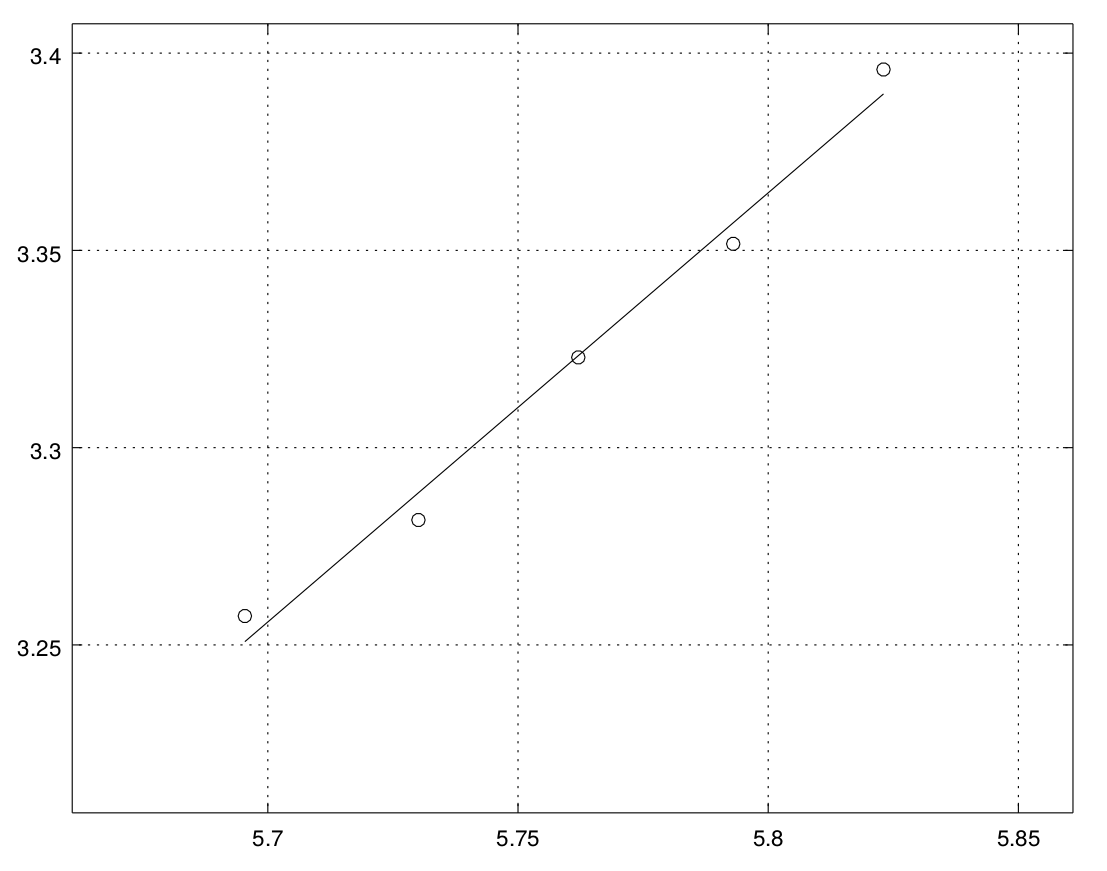
\includegraphics[scale=0.25]{zxc.png}
\end{figure}
\[
	\frac{d\left(\ln \varkappa\right)}{d\left(\ln T\right)} = 1.08
\]
\end{document}